\documentclass[12pt]{article}

\usepackage[T1]{fontenc}
\usepackage{mathpazo}
\usepackage{eulervm}

\usepackage{amsmath}
\usepackage{amsthm}
\allowdisplaybreaks[4]
\usepackage{amssymb}

\usepackage{tikz}
\usepackage{tikz-3dplot}
\usetikzlibrary{positioning}

\usetikzlibrary{decorations.pathreplacing, matrix}
\usepackage{nicematrix}
\usetikzlibrary{decorations.pathreplacing}
\usepackage{xy}  % Consider loading xy-pic only if needed

\usepackage{bm}
\usepackage{dcolumn} %  This package is for aligning numbers in columns, useful for tables.
\usepackage[mathscr]{eucal} % This package provides script fonts for mathematical calligraphic symbols.
\usepackage{float}  % For float placement control (e.g., [H] for "exactly here")
\usepackage{graphicx} % For including images

\usepackage{times} % This package is deprecated. Consider using a different font package if needed.
\usepackage{epstopdf} % For including EPS images (usually not needed with pdflatex)

\usepackage[square]{natbib} % Enables Author-Year citation style
\usepackage{bibentry}
\usepackage{cite} % For grouped citations like (1, 2, 3)


\usepackage{youngtab}  % For Young tableaux
\usepackage{ytableau}
\ytableausetup{mathmode, boxsize=0.9em}

\setlength{\evensidemargin}{0.3cm} % Consider unifying these lengths
\setlength{\oddsidemargin}{0.3cm}  % Consider unifying these lengths
\parskip=6pt
\frenchspacing
\textwidth=15cm
\textheight=23cm
\parindent=16pt
\topmargin=-1.2cm

% Theorem styles
\theoremstyle{definition}
\newtheorem{thm}{Theorem}[subsection]
\newtheorem{defi}[thm]{Definition}
\newtheorem{lemma}[thm]{Lemma}
\newtheorem{prop}[thm]{Proposition}
\newtheorem{coro}[thm]{Corollary}
\newtheorem{conj}[thm]{Conjecture}
\newtheorem*{pf}{Proof}

\newtheorem{ex}[thm]{Example}
\newtheorem{remark}[thm]{Remark}

\newtheorem{prob}{Problem}[subsection]

\numberwithin{equation}{subsection}

%\usepackage{hyperref}  % Load hyperref LAST (important!)


%-------------------------------------------------------------
\begin{document}


\begin{center}
{\Large\bf 
Notes on Volume Map
%and 
%Combinatorial Classes for \\[10pt]
%Restrictions of a Hyperplane Arrangement
}\\ [7pt]
\end{center}

\vskip 3mm

\begin{center}
Mingzhi Zhang
\end{center}

\vskip 3mm

\section{The "ellimination identity"}
Let 
\begin{align*}
    \Theta &=
\begin{bmatrix}
  \theta_1 \\
  \theta_2 \\
  \vdots \\
  \theta_d
\end{bmatrix} 
=
\begin{bmatrix}
  a_{11} & a_{12} & \ldots a_{1m} \\
  a_{21} & a_{22} & \ldots a_{2m} \\
  \vdots & \vdots & \vdots \\
  a_{d1} & a_{d2} & \ldots a_{dm} \\
\end{bmatrix} 
\begin{bmatrix}
  x_1 \\
  x_2 \\
  \vdots \\
  x_m
\end{bmatrix} \\
&:= \textbf{Mx} \\
&:=\sum_{i = 1}^{m} M_i x_i,
\end{align*}
\newline
and let $M_{\Theta}$ be the minor matrix whose colume vectors are $M_{i_1}$, $M_{i_2}$, $\ldots$, $M_{i_{d-1}}$, $\Theta$, where $i_1, i_2, \ldots, i_{d-1} \in [m]$.

Then we have that 
\begin{align*}
    \text{det}M_{\Theta} &= \text{det}(M_{i_{1}}, M_{i_{2}}, \ldots, M_{i_{d-1}}, \Theta) \\
    &= \text{det}(M_{i_{1}}, M_{i_{2}}, \ldots, M_{i_{d-1}}, \sum_{i = 1}^{m} M_i x_i) \\
    &= \sum_{i = 1}^{m} \text{det}(M_{i_{1}}, M_{i_{2}}, \ldots, M_{i_{d-1}}, M_i)  x_i
\end{align*}

Let \( \langle \Theta \rangle = \langle \theta_1, \theta_2, \ldots, \theta_d \rangle \) be the ideal generated by the \( \theta_i \)'s. It is direct to see that \( \det M_\Theta \in \langle \Theta \rangle \).

\section{The volume map}
Given a simplicial sphere $\Delta$ with vertices $[m]$ and suppose that $\text{dim }\Delta = d-1$.







\begin{center}
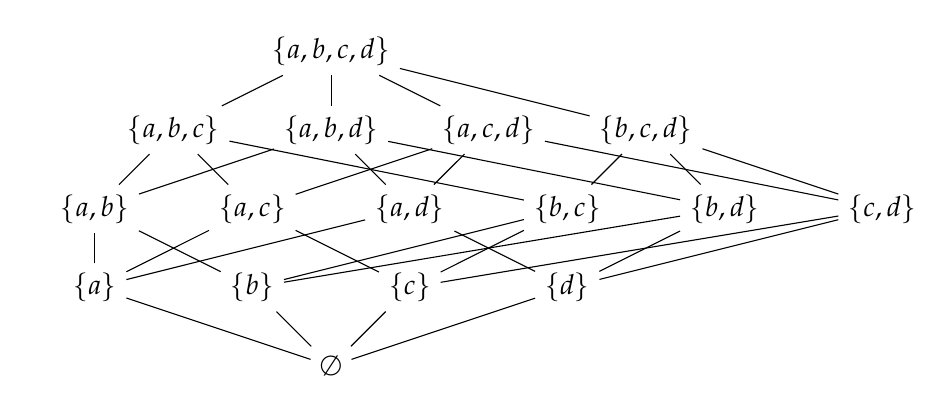
\begin{tikzpicture}
    % Nodes
    \node (top) at (0,4) {$\{a,b,c,d\}$};
    \node (abc) at (-2,3) {$\{a,b,c\}$};
    \node (abd) at (0,3) {$\{a,b,d\}$};
    \node (acd) at (2,3) {$\{a,c,d\}$};
    \node (bcd) at (4,3) {$\{b,c,d\}$};
    
    \node (ab) at (-3,2) {$\{a,b\}$};
    \node (ac) at (-1,2) {$\{a,c\}$};
    \node (ad) at (1,2) {$\{a,d\}$};
    \node (bc) at (3,2) {$\{b,c\}$};
    \node (bd) at (5,2) {$\{b,d\}$};
    \node (cd) at (7,2) {$\{c,d\}$};
    
    \node (a) at (-3,1) {$\{a\}$};
    \node (b) at (-1,1) {$\{b\}$};
    \node (c) at (1,1) {$\{c\}$};
    \node (d) at (3,1) {$\{d\}$};
    
    \node (bottom) at (0,0) {$\emptyset$};

    % Edges
    \draw (bottom) -- (a);
    \draw (bottom) -- (b);
    \draw (bottom) -- (c);
    \draw (bottom) -- (d);
    
    \draw (a) -- (ab);
    \draw (a) -- (ac);
    \draw (a) -- (ad);
    \draw (b) -- (ab);
    \draw (b) -- (bc);
    \draw (b) -- (bd);
    \draw (c) -- (ac);
    \draw (c) -- (bc);
    \draw (c) -- (cd);
    \draw (d) -- (ad);
    \draw (d) -- (bd);
    \draw (d) -- (cd);
    
    \draw (ab) -- (abc);
    \draw (ab) -- (abd);
    \draw (ac) -- (abc);
    \draw (ac) -- (acd);
    \draw (ad) -- (abd);
    \draw (ad) -- (acd);
    \draw (bc) -- (abc);
    \draw (bc) -- (bcd);
    \draw (bd) -- (abd);
    \draw (bd) -- (bcd);
    \draw (cd) -- (acd);
    \draw (cd) -- (bcd);
    
    \draw (abc) -- (top);
    \draw (abd) -- (top);
    \draw (acd) -- (top);
    \draw (bcd) -- (top);
\end{tikzpicture}
\end{center}


   






\begin{thebibliography}{99}
\raggedright
\bibitem[PP20]{PP20} Papadakis, Stavros Argyrios, and Vasiliki Petrotou. "The characteristic 2 anisotropicity of simplicial spheres." arXiv preprint arXiv:2012.09815 (2020).
\bibitem[AHK18]{AHK18} Adiprasito, Karim, June Huh, and Eric Katz. "Hodge theory for combinatorial geometries." Annals of Mathematics 188.2 (2018): 381-452.


\end{thebibliography}


\end{document}